\documentclass{article} % For LaTeX2e
\usepackage{iclr2019_conference,times}

% Optional math commands from https://github.com/goodfeli/dlbook_notation.
%%%%% NEW MATH DEFINITIONS %%%%%

\usepackage{amsmath,amsfonts,bm}

% Mark sections of captions for referring to divisions of figures
\newcommand{\figleft}{{\em (Left)}}
\newcommand{\figcenter}{{\em (Center)}}
\newcommand{\figright}{{\em (Right)}}
\newcommand{\figtop}{{\em (Top)}}
\newcommand{\figbottom}{{\em (Bottom)}}
\newcommand{\captiona}{{\em (a)}}
\newcommand{\captionb}{{\em (b)}}
\newcommand{\captionc}{{\em (c)}}
\newcommand{\captiond}{{\em (d)}}

% Highlight a newly defined term
\newcommand{\newterm}[1]{{\bf #1}}


% Figure reference, lower-case.
\def\figref#1{figure~\ref{#1}}
% Figure reference, capital. For start of sentence
\def\Figref#1{Figure~\ref{#1}}
\def\twofigref#1#2{figures \ref{#1} and \ref{#2}}
\def\quadfigref#1#2#3#4{figures \ref{#1}, \ref{#2}, \ref{#3} and \ref{#4}}
% Section reference, lower-case.
\def\secref#1{section~\ref{#1}}
% Section reference, capital.
\def\Secref#1{Section~\ref{#1}}
% Reference to two sections.
\def\twosecrefs#1#2{sections \ref{#1} and \ref{#2}}
% Reference to three sections.
\def\secrefs#1#2#3{sections \ref{#1}, \ref{#2} and \ref{#3}}
% Reference to an equation, lower-case.
\def\eqref#1{equation~\ref{#1}}
% Reference to an equation, upper case
\def\Eqref#1{Equation~\ref{#1}}
% A raw reference to an equation---avoid using if possible
\def\plaineqref#1{\ref{#1}}
% Reference to a chapter, lower-case.
\def\chapref#1{chapter~\ref{#1}}
% Reference to an equation, upper case.
\def\Chapref#1{Chapter~\ref{#1}}
% Reference to a range of chapters
\def\rangechapref#1#2{chapters\ref{#1}--\ref{#2}}
% Reference to an algorithm, lower-case.
\def\algref#1{algorithm~\ref{#1}}
% Reference to an algorithm, upper case.
\def\Algref#1{Algorithm~\ref{#1}}
\def\twoalgref#1#2{algorithms \ref{#1} and \ref{#2}}
\def\Twoalgref#1#2{Algorithms \ref{#1} and \ref{#2}}
% Reference to a part, lower case
\def\partref#1{part~\ref{#1}}
% Reference to a part, upper case
\def\Partref#1{Part~\ref{#1}}
\def\twopartref#1#2{parts \ref{#1} and \ref{#2}}

\def\ceil#1{\lceil #1 \rceil}
\def\floor#1{\lfloor #1 \rfloor}
\def\1{\bm{1}}
\newcommand{\train}{\mathcal{D}}
\newcommand{\valid}{\mathcal{D_{\mathrm{valid}}}}
\newcommand{\test}{\mathcal{D_{\mathrm{test}}}}

\def\eps{{\epsilon}}


% Random variables
\def\reta{{\textnormal{$\eta$}}}
\def\ra{{\textnormal{a}}}
\def\rb{{\textnormal{b}}}
\def\rc{{\textnormal{c}}}
\def\rd{{\textnormal{d}}}
\def\re{{\textnormal{e}}}
\def\rf{{\textnormal{f}}}
\def\rg{{\textnormal{g}}}
\def\rh{{\textnormal{h}}}
\def\ri{{\textnormal{i}}}
\def\rj{{\textnormal{j}}}
\def\rk{{\textnormal{k}}}
\def\rl{{\textnormal{l}}}
% rm is already a command, just don't name any random variables m
\def\rn{{\textnormal{n}}}
\def\ro{{\textnormal{o}}}
\def\rp{{\textnormal{p}}}
\def\rq{{\textnormal{q}}}
\def\rr{{\textnormal{r}}}
\def\rs{{\textnormal{s}}}
\def\rt{{\textnormal{t}}}
\def\ru{{\textnormal{u}}}
\def\rv{{\textnormal{v}}}
\def\rw{{\textnormal{w}}}
\def\rx{{\textnormal{x}}}
\def\ry{{\textnormal{y}}}
\def\rz{{\textnormal{z}}}

% Random vectors
\def\rvepsilon{{\mathbf{\epsilon}}}
\def\rvtheta{{\mathbf{\theta}}}
\def\rva{{\mathbf{a}}}
\def\rvb{{\mathbf{b}}}
\def\rvc{{\mathbf{c}}}
\def\rvd{{\mathbf{d}}}
\def\rve{{\mathbf{e}}}
\def\rvf{{\mathbf{f}}}
\def\rvg{{\mathbf{g}}}
\def\rvh{{\mathbf{h}}}
\def\rvu{{\mathbf{i}}}
\def\rvj{{\mathbf{j}}}
\def\rvk{{\mathbf{k}}}
\def\rvl{{\mathbf{l}}}
\def\rvm{{\mathbf{m}}}
\def\rvn{{\mathbf{n}}}
\def\rvo{{\mathbf{o}}}
\def\rvp{{\mathbf{p}}}
\def\rvq{{\mathbf{q}}}
\def\rvr{{\mathbf{r}}}
\def\rvs{{\mathbf{s}}}
\def\rvt{{\mathbf{t}}}
\def\rvu{{\mathbf{u}}}
\def\rvv{{\mathbf{v}}}
\def\rvw{{\mathbf{w}}}
\def\rvx{{\mathbf{x}}}
\def\rvy{{\mathbf{y}}}
\def\rvz{{\mathbf{z}}}

% Elements of random vectors
\def\erva{{\textnormal{a}}}
\def\ervb{{\textnormal{b}}}
\def\ervc{{\textnormal{c}}}
\def\ervd{{\textnormal{d}}}
\def\erve{{\textnormal{e}}}
\def\ervf{{\textnormal{f}}}
\def\ervg{{\textnormal{g}}}
\def\ervh{{\textnormal{h}}}
\def\ervi{{\textnormal{i}}}
\def\ervj{{\textnormal{j}}}
\def\ervk{{\textnormal{k}}}
\def\ervl{{\textnormal{l}}}
\def\ervm{{\textnormal{m}}}
\def\ervn{{\textnormal{n}}}
\def\ervo{{\textnormal{o}}}
\def\ervp{{\textnormal{p}}}
\def\ervq{{\textnormal{q}}}
\def\ervr{{\textnormal{r}}}
\def\ervs{{\textnormal{s}}}
\def\ervt{{\textnormal{t}}}
\def\ervu{{\textnormal{u}}}
\def\ervv{{\textnormal{v}}}
\def\ervw{{\textnormal{w}}}
\def\ervx{{\textnormal{x}}}
\def\ervy{{\textnormal{y}}}
\def\ervz{{\textnormal{z}}}

% Random matrices
\def\rmA{{\mathbf{A}}}
\def\rmB{{\mathbf{B}}}
\def\rmC{{\mathbf{C}}}
\def\rmD{{\mathbf{D}}}
\def\rmE{{\mathbf{E}}}
\def\rmF{{\mathbf{F}}}
\def\rmG{{\mathbf{G}}}
\def\rmH{{\mathbf{H}}}
\def\rmI{{\mathbf{I}}}
\def\rmJ{{\mathbf{J}}}
\def\rmK{{\mathbf{K}}}
\def\rmL{{\mathbf{L}}}
\def\rmM{{\mathbf{M}}}
\def\rmN{{\mathbf{N}}}
\def\rmO{{\mathbf{O}}}
\def\rmP{{\mathbf{P}}}
\def\rmQ{{\mathbf{Q}}}
\def\rmR{{\mathbf{R}}}
\def\rmS{{\mathbf{S}}}
\def\rmT{{\mathbf{T}}}
\def\rmU{{\mathbf{U}}}
\def\rmV{{\mathbf{V}}}
\def\rmW{{\mathbf{W}}}
\def\rmX{{\mathbf{X}}}
\def\rmY{{\mathbf{Y}}}
\def\rmZ{{\mathbf{Z}}}

% Elements of random matrices
\def\ermA{{\textnormal{A}}}
\def\ermB{{\textnormal{B}}}
\def\ermC{{\textnormal{C}}}
\def\ermD{{\textnormal{D}}}
\def\ermE{{\textnormal{E}}}
\def\ermF{{\textnormal{F}}}
\def\ermG{{\textnormal{G}}}
\def\ermH{{\textnormal{H}}}
\def\ermI{{\textnormal{I}}}
\def\ermJ{{\textnormal{J}}}
\def\ermK{{\textnormal{K}}}
\def\ermL{{\textnormal{L}}}
\def\ermM{{\textnormal{M}}}
\def\ermN{{\textnormal{N}}}
\def\ermO{{\textnormal{O}}}
\def\ermP{{\textnormal{P}}}
\def\ermQ{{\textnormal{Q}}}
\def\ermR{{\textnormal{R}}}
\def\ermS{{\textnormal{S}}}
\def\ermT{{\textnormal{T}}}
\def\ermU{{\textnormal{U}}}
\def\ermV{{\textnormal{V}}}
\def\ermW{{\textnormal{W}}}
\def\ermX{{\textnormal{X}}}
\def\ermY{{\textnormal{Y}}}
\def\ermZ{{\textnormal{Z}}}

% Vectors
\def\vzero{{\bm{0}}}
\def\vone{{\bm{1}}}
\def\vmu{{\bm{\mu}}}
\def\vtheta{{\bm{\theta}}}
\def\va{{\bm{a}}}
\def\vb{{\bm{b}}}
\def\vc{{\bm{c}}}
\def\vd{{\bm{d}}}
\def\ve{{\bm{e}}}
\def\vf{{\bm{f}}}
\def\vg{{\bm{g}}}
\def\vh{{\bm{h}}}
\def\vi{{\bm{i}}}
\def\vj{{\bm{j}}}
\def\vk{{\bm{k}}}
\def\vl{{\bm{l}}}
\def\vm{{\bm{m}}}
\def\vn{{\bm{n}}}
\def\vo{{\bm{o}}}
\def\vp{{\bm{p}}}
\def\vq{{\bm{q}}}
\def\vr{{\bm{r}}}
\def\vs{{\bm{s}}}
\def\vt{{\bm{t}}}
\def\vu{{\bm{u}}}
\def\vv{{\bm{v}}}
\def\vw{{\bm{w}}}
\def\vx{{\bm{x}}}
\def\vy{{\bm{y}}}
\def\vz{{\bm{z}}}

% Elements of vectors
\def\evalpha{{\alpha}}
\def\evbeta{{\beta}}
\def\evepsilon{{\epsilon}}
\def\evlambda{{\lambda}}
\def\evomega{{\omega}}
\def\evmu{{\mu}}
\def\evpsi{{\psi}}
\def\evsigma{{\sigma}}
\def\evtheta{{\theta}}
\def\eva{{a}}
\def\evb{{b}}
\def\evc{{c}}
\def\evd{{d}}
\def\eve{{e}}
\def\evf{{f}}
\def\evg{{g}}
\def\evh{{h}}
\def\evi{{i}}
\def\evj{{j}}
\def\evk{{k}}
\def\evl{{l}}
\def\evm{{m}}
\def\evn{{n}}
\def\evo{{o}}
\def\evp{{p}}
\def\evq{{q}}
\def\evr{{r}}
\def\evs{{s}}
\def\evt{{t}}
\def\evu{{u}}
\def\evv{{v}}
\def\evw{{w}}
\def\evx{{x}}
\def\evy{{y}}
\def\evz{{z}}

% Matrix
\def\mA{{\bm{A}}}
\def\mB{{\bm{B}}}
\def\mC{{\bm{C}}}
\def\mD{{\bm{D}}}
\def\mE{{\bm{E}}}
\def\mF{{\bm{F}}}
\def\mG{{\bm{G}}}
\def\mH{{\bm{H}}}
\def\mI{{\bm{I}}}
\def\mJ{{\bm{J}}}
\def\mK{{\bm{K}}}
\def\mL{{\bm{L}}}
\def\mM{{\bm{M}}}
\def\mN{{\bm{N}}}
\def\mO{{\bm{O}}}
\def\mP{{\bm{P}}}
\def\mQ{{\bm{Q}}}
\def\mR{{\bm{R}}}
\def\mS{{\bm{S}}}
\def\mT{{\bm{T}}}
\def\mU{{\bm{U}}}
\def\mV{{\bm{V}}}
\def\mW{{\bm{W}}}
\def\mX{{\bm{X}}}
\def\mY{{\bm{Y}}}
\def\mZ{{\bm{Z}}}
\def\mBeta{{\bm{\beta}}}
\def\mPhi{{\bm{\Phi}}}
\def\mLambda{{\bm{\Lambda}}}
\def\mSigma{{\bm{\Sigma}}}

% Tensor
\DeclareMathAlphabet{\mathsfit}{\encodingdefault}{\sfdefault}{m}{sl}
\SetMathAlphabet{\mathsfit}{bold}{\encodingdefault}{\sfdefault}{bx}{n}
\newcommand{\tens}[1]{\bm{\mathsfit{#1}}}
\def\tA{{\tens{A}}}
\def\tB{{\tens{B}}}
\def\tC{{\tens{C}}}
\def\tD{{\tens{D}}}
\def\tE{{\tens{E}}}
\def\tF{{\tens{F}}}
\def\tG{{\tens{G}}}
\def\tH{{\tens{H}}}
\def\tI{{\tens{I}}}
\def\tJ{{\tens{J}}}
\def\tK{{\tens{K}}}
\def\tL{{\tens{L}}}
\def\tM{{\tens{M}}}
\def\tN{{\tens{N}}}
\def\tO{{\tens{O}}}
\def\tP{{\tens{P}}}
\def\tQ{{\tens{Q}}}
\def\tR{{\tens{R}}}
\def\tS{{\tens{S}}}
\def\tT{{\tens{T}}}
\def\tU{{\tens{U}}}
\def\tV{{\tens{V}}}
\def\tW{{\tens{W}}}
\def\tX{{\tens{X}}}
\def\tY{{\tens{Y}}}
\def\tZ{{\tens{Z}}}


% Graph
\def\gA{{\mathcal{A}}}
\def\gB{{\mathcal{B}}}
\def\gC{{\mathcal{C}}}
\def\gD{{\mathcal{D}}}
\def\gE{{\mathcal{E}}}
\def\gF{{\mathcal{F}}}
\def\gG{{\mathcal{G}}}
\def\gH{{\mathcal{H}}}
\def\gI{{\mathcal{I}}}
\def\gJ{{\mathcal{J}}}
\def\gK{{\mathcal{K}}}
\def\gL{{\mathcal{L}}}
\def\gM{{\mathcal{M}}}
\def\gN{{\mathcal{N}}}
\def\gO{{\mathcal{O}}}
\def\gP{{\mathcal{P}}}
\def\gQ{{\mathcal{Q}}}
\def\gR{{\mathcal{R}}}
\def\gS{{\mathcal{S}}}
\def\gT{{\mathcal{T}}}
\def\gU{{\mathcal{U}}}
\def\gV{{\mathcal{V}}}
\def\gW{{\mathcal{W}}}
\def\gX{{\mathcal{X}}}
\def\gY{{\mathcal{Y}}}
\def\gZ{{\mathcal{Z}}}

% Sets
\def\sA{{\mathbb{A}}}
\def\sB{{\mathbb{B}}}
\def\sC{{\mathbb{C}}}
\def\sD{{\mathbb{D}}}
% Don't use a set called E, because this would be the same as our symbol
% for expectation.
\def\sF{{\mathbb{F}}}
\def\sG{{\mathbb{G}}}
\def\sH{{\mathbb{H}}}
\def\sI{{\mathbb{I}}}
\def\sJ{{\mathbb{J}}}
\def\sK{{\mathbb{K}}}
\def\sL{{\mathbb{L}}}
\def\sM{{\mathbb{M}}}
\def\sN{{\mathbb{N}}}
\def\sO{{\mathbb{O}}}
\def\sP{{\mathbb{P}}}
\def\sQ{{\mathbb{Q}}}
\def\sR{{\mathbb{R}}}
\def\sS{{\mathbb{S}}}
\def\sT{{\mathbb{T}}}
\def\sU{{\mathbb{U}}}
\def\sV{{\mathbb{V}}}
\def\sW{{\mathbb{W}}}
\def\sX{{\mathbb{X}}}
\def\sY{{\mathbb{Y}}}
\def\sZ{{\mathbb{Z}}}

% Entries of a matrix
\def\emLambda{{\Lambda}}
\def\emA{{A}}
\def\emB{{B}}
\def\emC{{C}}
\def\emD{{D}}
\def\emE{{E}}
\def\emF{{F}}
\def\emG{{G}}
\def\emH{{H}}
\def\emI{{I}}
\def\emJ{{J}}
\def\emK{{K}}
\def\emL{{L}}
\def\emM{{M}}
\def\emN{{N}}
\def\emO{{O}}
\def\emP{{P}}
\def\emQ{{Q}}
\def\emR{{R}}
\def\emS{{S}}
\def\emT{{T}}
\def\emU{{U}}
\def\emV{{V}}
\def\emW{{W}}
\def\emX{{X}}
\def\emY{{Y}}
\def\emZ{{Z}}
\def\emSigma{{\Sigma}}

% entries of a tensor
% Same font as tensor, without \bm wrapper
\newcommand{\etens}[1]{\mathsfit{#1}}
\def\etLambda{{\etens{\Lambda}}}
\def\etA{{\etens{A}}}
\def\etB{{\etens{B}}}
\def\etC{{\etens{C}}}
\def\etD{{\etens{D}}}
\def\etE{{\etens{E}}}
\def\etF{{\etens{F}}}
\def\etG{{\etens{G}}}
\def\etH{{\etens{H}}}
\def\etI{{\etens{I}}}
\def\etJ{{\etens{J}}}
\def\etK{{\etens{K}}}
\def\etL{{\etens{L}}}
\def\etM{{\etens{M}}}
\def\etN{{\etens{N}}}
\def\etO{{\etens{O}}}
\def\etP{{\etens{P}}}
\def\etQ{{\etens{Q}}}
\def\etR{{\etens{R}}}
\def\etS{{\etens{S}}}
\def\etT{{\etens{T}}}
\def\etU{{\etens{U}}}
\def\etV{{\etens{V}}}
\def\etW{{\etens{W}}}
\def\etX{{\etens{X}}}
\def\etY{{\etens{Y}}}
\def\etZ{{\etens{Z}}}

% The true underlying data generating distribution
\newcommand{\pdata}{p_{\rm{data}}}
% The empirical distribution defined by the training set
\newcommand{\ptrain}{\hat{p}_{\rm{data}}}
\newcommand{\Ptrain}{\hat{P}_{\rm{data}}}
% The model distribution
\newcommand{\pmodel}{p_{\rm{model}}}
\newcommand{\Pmodel}{P_{\rm{model}}}
\newcommand{\ptildemodel}{\tilde{p}_{\rm{model}}}
% Stochastic autoencoder distributions
\newcommand{\pencode}{p_{\rm{encoder}}}
\newcommand{\pdecode}{p_{\rm{decoder}}}
\newcommand{\precons}{p_{\rm{reconstruct}}}

\newcommand{\laplace}{\mathrm{Laplace}} % Laplace distribution

\newcommand{\E}{\mathbb{E}}
\newcommand{\Ls}{\mathcal{L}}
\newcommand{\R}{\mathbb{R}}
\newcommand{\emp}{\tilde{p}}
\newcommand{\lr}{\alpha}
\newcommand{\reg}{\lambda}
\newcommand{\rect}{\mathrm{rectifier}}
\newcommand{\softmax}{\mathrm{softmax}}
\newcommand{\sigmoid}{\sigma}
\newcommand{\softplus}{\zeta}
\newcommand{\KL}{D_{\mathrm{KL}}}
\newcommand{\Var}{\mathrm{Var}}
\newcommand{\standarderror}{\mathrm{SE}}
\newcommand{\Cov}{\mathrm{Cov}}
% Wolfram Mathworld says $L^2$ is for function spaces and $\ell^2$ is for vectors
% But then they seem to use $L^2$ for vectors throughout the site, and so does
% wikipedia.
\newcommand{\normlzero}{L^0}
\newcommand{\normlone}{L^1}
\newcommand{\normltwo}{L^2}
\newcommand{\normlp}{L^p}
\newcommand{\normmax}{L^\infty}

\newcommand{\parents}{Pa} % See usage in notation.tex. Chosen to match Daphne's book.

\DeclareMathOperator*{\argmax}{arg\,max}
\DeclareMathOperator*{\argmin}{arg\,min}

\DeclareMathOperator{\sign}{sign}
\DeclareMathOperator{\Tr}{Tr}
\let\ab\allowbreak


\usepackage{hyperref}
\usepackage{url}
\usepackage{graphicx}


\title{Reproducibility Challenge: \\ Deep Learning for Symbolic Mathematics}

% Authors must not appear in the submitted version. They should be hidden
% as long as the \iclrfinalcopy macro remains commented out below.
% Non-anonymous submissions will be rejected without review.

\author{Xiaoxuan Wu, Ruixue Guo, Zeliang Zhao \& Wanyuan Lin\\
School of Electronics \& Computer Science\\
University of Southampton\\
\texttt{\{xw5u21,rg6g21,zz8u21,wl7n21\}@soton.ac.uk}
}


\newcommand{\fix}{\marginpar{FIX}}
\newcommand{\new}{\marginpar{NEW}}

\iclrfinalcopy % Uncomment for camera-ready version, but NOT for submission.
\begin{document}


\maketitle

\begin{abstract}
It has been proved in \textit {Deep Learning for Symbolic Mathematics} \citet{Lample} that neural networks perform good on mathematical tasks. This project aims to re-implement parts of the experiments established in that paper and analyse its reproducibility. The code of our experiment is available at \url{https://github.com/cora0305/COMP6248-Reproducability-Challenge}.
\end{abstract}

\section{Introduction}
At a time when neural networks are widely used, people have relatively little attention on considering using it to solve mathematical problems such as symbolic calculations. Moreover, among existing studies on this topic, the majority of  them treat it as arithmetic tasks like integer addition and multiplication\cite{zaremba2014learning, arabshahi2018towards}. The original paper proposed the method to consider symbolic calculations as a target for NLP models and utilise sequence-to-sequence models (seq2seq) to solve this problem. Our team reproduced some key experiments and the details are as follows.


\section{Method \& Algorithm}
\label{MnA}
In the original paper, the authors’ main ideas are divided into three parts: generate data, train the model, and predict results. The first step is to generate data so that the deep learning model is a large number of known samples to do the training. The second step of training the model is to use the data from the first step to train the seq2seq model. The third step is to predict the outcome given a function or a differential equation, use the model that has been trained to predict the outcome, rank the multiple outcomes predicted, and choose the most likely one as the value for the symbolic calculation.

\subsection{Expression as Trees}
Before using the seq2seq models to finish the task, it is necessary to convert mathematical expressions to trees and from trees to sequences, with operators and internal nodes, children, numbers, constants, and variables as leaves. %The following trees (Figure 1) represent expressions $2+3\times(5+2)$, $3x^2+cos(2x)-1$, and $\frac{\partial^{2} \psi}{\partial x^{2}}-\frac{1}{\upsilon^{2}} \frac{\partial^{2} \psi}{\partial t^{2}}$:
%\begin{figure}[h]
%\begin{center}
%%\framebox[4.0in]{$\;$}
%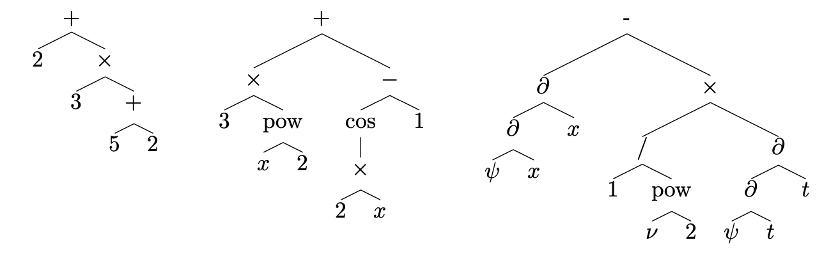
\includegraphics[height=0.2\textwidth]{figures/expressionastree.png}
%%\fbox{\rule[-.5cm]{0cm}{4cm} \rule[-.5cm]{4cm}{0cm}}
%\end{center}
%\caption{Expression as tress}
%\end{figure}

\subsection{Data Generation}
Before generating the data, the authors placed the necessary restrictions on the scope of the data:\\
$\bullet$ \quad expression with up to the $n=15$ internal nodes\\
$\bullet$ \quad $L=11$ leaf values in $\{x\}\cup\{-5, \ldots, 5\} \backslash\{0\}$\\
$\bullet$ \quad $p_{2}=4$ binary operators: $+,-,\times,/$\\
$\bullet$ \quad $p_{1}=15$ unary operators:\\
$\exp, \log$, sqrt, $\sin, \cos, \tan, \sin ^{-1}, \cos ^{-1}, \tan ^{-1}, \sinh , \cosh , \tanh , \sinh ^{-1}, \cosh h^{-1}, \tanh ^{-1}$\\
The original paper used three approaches to data generation, respectively Forward Generation (FWD), Backward Generation (BWD), and Backward Generation with Integration by Parts (IBP).

Forward Generation (FWD):
$$\stackrel{\text { Generate }}{\longrightarrow} f \stackrel{\text { Integrate }}{\longrightarrow} F$$
This approach generates a random function $f$, computes its antiderivative $F$ using an external symbolic framework (Sympy, Mathematica, etc.), and adds $(f,F)$ to the training set.

Backward Generation (BWD):
$$f \stackrel{\text { Differentiate }}{\longleftarrow} F \stackrel{\text { Generate }}{\longleftarrow}$$
This approach generates a function $F$, computes its derivative, and adds $(f,F)$ to the training set.\\
BWD leads to long problems with short solutions whereas FWD leads to short problems with longer solutions.

Integration by Parts (IBP):\\
This approach generates random functions $F$ and $G$, computes their derivatives $f$ and $g$ and if $f*G$ is in the training set, computes the integral of $F*g$ with $\int F g=F G-\int f G$.\\
In our task, we used the first two approaches (FWD and BWD) to generate data.

\subsection{Model}
$\bullet$ \quad seq2seq model\\
The seq2seq model is converting a sequence signal as an input into an output sequence signal. Using a deep neural network, the process consists of two processes: encoding and decoding.

$\bullet$ \quad Transformer model\\
The transformer model is a seq2seq model \cite{vaswani2017attention}.The architecture of transformer model is below (Figure \ref{trans_archi}). It contains two parts, the Encoder, and the Decoder. Unlike the original seq2seq model, there is no RNN in the transformer model, which is entirely based on Attention and fully connected layers.
% \begin{figure}[h]
% \begin{center}
% 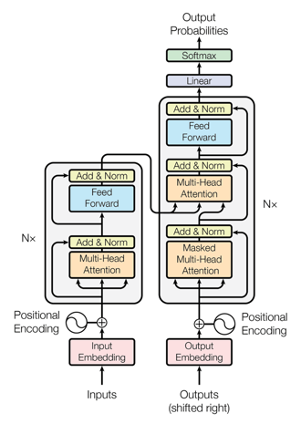
\includegraphics[height=0.5\textwidth]{figures/transformermodelarchi.png}
% \end{center}
% \caption{The transformer model architecture }
% \label{trans_archi}
% \end{figure}
% In this task, we used a transformer model the same as the original paper with 8 attention heads, 6 layers, and dimensionality of 512. And we trained this model with the Adam optimizer with $10^{-4}$ learning rate.

\section{Implementation details}
\label{Implement}
\subsection{Dataset}
Basing the original paper, the implementation could be divided into two parts, the first one using the polynomial dataset and generated with the forward method, the second method using the BWD dataset \footnote{\url{https://dl.fbaipublicfiles.com/SymbolicMathematics/data/prim_bwd.tar.gz}} prepared from author that the task of integration and generated with the backward method.

\subsection{Baseline of the models}
The baseline of the models is same as the original paper, implementing the seq2seq model, using the default PyTorch's Transformer Encoder, Transformer Decoder module. Setting the learning rate with 0.0001, number of attentions of 8, number of encoder layer of 6, number of decoder layer of 6, model dimension of 512, and the Adam optimizer. Evaluating the performance of the model after each epoch on test and validation set. For evaluation, it simply compared the generated and target sequence. At inference, however, using sympy to compute the difference between the derivative of the generated primitive and the input. If there is no difference, it considers it as a valid answer.

\subsection{Forward method with polynomial dataset}
\label{implement_fwd}
By using the virtual machine prepared from ECS CAD Server, running the code in the GPU which Perf is P2 and the Pwr is P2. The environment is set with python 3.7, generating the data with the package sympy, building the model with PyTorch, and then training with PyTorch. Firstly, using the \texttt{data\_gen.py} to generate the polynomial data setting with different numbers, such as 1000, 10000 and so on. As the limit of the GPU machine, we only run the dataset with the number about 100000. It is very slow with a dataset of 100000 numbers. Then, running the \texttt{train.py} file to check the result of the loss, this step becomes faster with the forward method.

\subsection{Backward method with integration dataset}
By using the Google Colab virtual machine, running the code with the GPU that Tesla 48C. The environment is building with the file author prepared 'environment.yml', setting the environment with python 3.8, and the channels with PyTorch, anaconda and so on.\\
After activating the environment with the file, running the \texttt{main.py} with the different epoch sizes, batch sizes, epochs, training set and test set. Also, with the limit with the GPU, Tesla 48C could not run with the original dataset about 5000000 numbers, the maximum training set of the implementation is 1000000 numbers. Totally, running the five experiments with the different settings, the average time of each experiment is about 3-4 hours. Finally, the output results could be found with the generated log files in detail.

\section{Result \& Analysis}
\label{RnA}
\subsection{RESULTS OF BWD DATASET}

\begin{table}[h]
\caption{Results of BWD Data}
\label{bwd_result}
\begin{center}
\begin{tabular}{lllllllll}
\textbf{\begin{tabular}[c]{@{}l@{}}Experiment \\ Number\end{tabular}} &
  \textbf{\begin{tabular}[c]{@{}l@{}}Epoch\\ Size\end{tabular}} &
  \textbf{\begin{tabular}[c]{@{}l@{}}Batch\\ Size\end{tabular}} &
  \textbf{\begin{tabular}[c]{@{}l@{}}Epoch\\ Number\end{tabular}} &
  \textbf{\begin{tabular}[c]{@{}l@{}}Train\\ Size\end{tabular}} &
  \textbf{\begin{tabular}[c]{@{}l@{}}Test\\ Size\end{tabular}} &
  \textbf{\begin{tabular}[c]{@{}l@{}}Valid\\ Size\end{tabular}} &
  \textbf{\begin{tabular}[c]{@{}l@{}}Running\\ Time\\ (GPU)\end{tabular}} &
  \textbf{Accuracy} \\
\\ \hline \\
\#1 & 1024   & 32  & 30 & 1024    & 32  & 32  & 0:02:24 & 0.0\% \\
\#2 & 10000  & 32  & 30 & 10000   & 32  & 32  & 2:58:22 & 28.1\% \\
\#3 & 10000  & 32  & 30 & 10000   & 128 & 128 & 1:45:26 & 12.5\% \\
\#4 & 10000  & 32  & 40 & 10000   & 32  & 32  & 2:07:28 & 46.9\% \\
\#5 & 100000 & 32  & 30 & 1000000 & 500 & 500 & 4:28:37 & 95.4\% 
\end{tabular}
\end{center}
\end{table}

As shown in Table \ref{bwd_result}, Experiment 1 was an attempt to figure out the model complexity. The accuracy is 0.0\% since the number of training set is too small. As shown in Experiment 2, the accuracy improves as the number of training sample increases.

Comparing the results of Experiment 2 and 3, it shows that the model will perform poorly if only increasing the number of test and validation set without increasing the number of training set with the same order of magnitude. From the previous experimental results, it is known that the accuracy is relatively high only when the ratio of training size and test size is large.

Further, by comparing Experiment 4 and 2, the accuracy is almost doubled by increasing the epoch number while maintaining the size of training and test sets. However, both the test and validation accuracy are unstable as shown in Figure \ref{fluctuations}. This issue will be addressed in the following experiment by increasing the number of training set.

\begin{figure}[h]
\begin{minipage}[t]{0.45\linewidth}
\centering
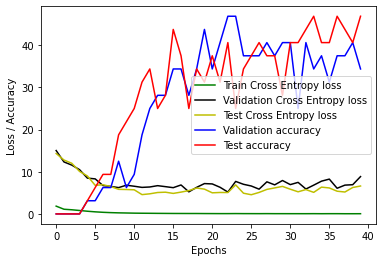
\includegraphics[width=5.5cm,height=3.5cm]{figures/F1.png}
\caption{Fluctuations of Accuracy}
\label{fluctuations}
\end{minipage}
\begin{minipage}[t]{0.45\linewidth}
\hspace{15pt}
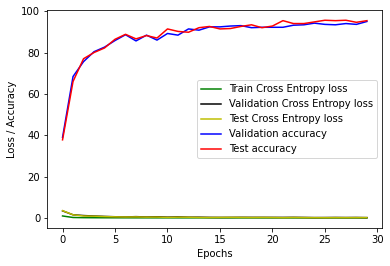
\includegraphics[width=5.5cm,height=3.5cm]{figures/F2.png}
\caption{Final Result}
\label{finalResult}
\end{minipage}
\end{figure}

Figure \ref{finalResult} presents the plot of Experiment 5. It can be observed that the accuracy is stable and steadily increasing with each subsequent epoch finally reaching 95.4\%. It is promising to achieve the 98.4\% accuracy, which is implemented by the original paper, by increasing the sizes of training and test samples accordingly. Therefore, this is considered to be a successful reproduction of part of the original paper.

\subsection{RESULTS OF FWD DATASET}

\begin{table}[h]
\caption{Results of FWD Data}
\label{fwd_result}
\begin{center}
\begin{tabular}{llll}
\textbf{Data} & \textbf{Batch Size} & \textbf{Epoch} & \textbf{Loss}\\
\\ \hline \\
100 & 64 & 20 & 0.52101 \\
500 & 64  & 200  & 0.04062 \\
1000 & 64  & 200  & 0.00804 \\
10000 & 64  & 100  & 0.00983 \\
10000 & 64 & 200  & 0.00347 \\
100000 & 32 & 10  & 0.01900 \\
100000 & 64 & 100  & 0.00958 \\
\end{tabular}
\end{center}
\end{table}

Table \ref{fwd_result} shows the results of FWD dataset. The trends of results are similar to those of BWD dataset, so it will not be described again. Notably, instead of using the given data, new data generated here by ourselves was used as the training set.

As mentioned in Section \ref{implement_fwd}, the maximum 100,000 data were generated and trained with 100 epochs which took more than 27 hours. Due to the computing power of available GPU, this is the limit of the experiment that can be conducted.

\section{Conclusion}
In this task, we show that the machine translation model is suitable for symbolic mathematic tasks, and the seq2seq model can be used for difficult tasks like function integration. We use Forward Generation (FWD) to generate polynomials and express them as sum of powers. We use Backward Generation (BWD) to generate data and calculate the integration. After experiments, we show that the 6th experiment (100,000 epoch size, 32 batch size, 1,000,000 training size) has the best performance with the accuracy of 95.4\%. \\
This approach takes advantage of neural networks to reconstruct mathematical problems based on translating some of math’s complicated equations with the seq2seq model.

\bibliography{iclr2019_conference}
\bibliographystyle{iclr2019_conference}

\end{document}
